\documentclass[11pt]{article}
\usepackage{fullpage}
\usepackage{setspace}
\usepackage{amsmath}
\usepackage{fancyvrb}
\usepackage{enumerate}
\usepackage{listings}
\usepackage{pgfplots}
\usepackage{graphicx}
\usepackage{float}
\usepackage{multirow}
\usepackage[format=hang,labelsep=quad]{caption}
\usepackage{subfig}
\usepackage{array}
\usepackage{multirow}

\renewcommand\thesubfigure{\roman{subfigure}}


\begin{document}
\noindent\large{Math 5364}\\
\large{Data Mining 2}\\
\large{Homework 23}\\
\large{Mary Barker}
\doublespace

\begin{enumerate}
\item 
Import the file math5305Lab6Data.txt, whose columns are the variables 
Y, X1, X2, and X3. The goal of these first three problems is to 
perform diagnostics to assess the assumptions of normality and constancy 
of variabce for a model predicting Y from the Xj's, to transform Y if 
necessary, to assess the transformed model using diagnostics, adn to 
compare the original and transformed models via residual sums of squares. 

We begin by fitting a model and assessing it with diagnostics. 

\begin{enumerate}
\item 
Fit model = lm(Y~X1+X2+X3), compute the fitted values Yhat, and the 
residuals e. You can use the command Yhat = predict(model) to obtain 
Yhat. 

\item 
Plot Y vs Yhat. If the model were valid, what would you expect this 
plot to look like? Does the plot suggest the existence of curvature 
in the model? 

If this were a valid model, then the predictions $\hat{Y}$ would be 
roughly equal to the $Y$ values. Therefore the plot of $\hat{Y}$ vs 
$Y$ for a valid model should be a diagonal line. 

\begin{center}
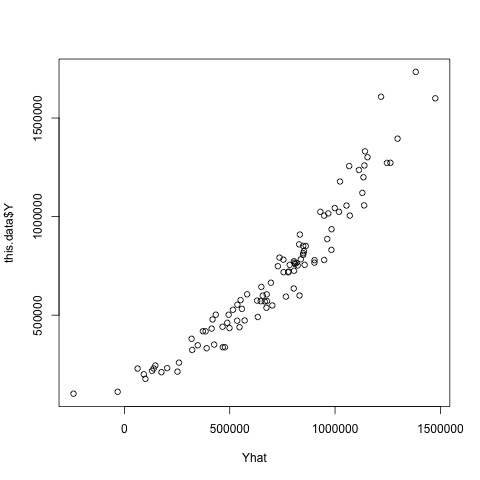
\includegraphics[width=0.5\textwidth]{Yhat_vs_Y}
\end{center}

The plot does have a mainly diagonal line, but the curvature suggests 
that the model is not accurately representing some relationship in the 
predictor variables. 

\item 
Plot e vs Yhat. If the model were valid, what would you expect this 
plot to look like? Does the plot suggest the existence of curvature 
in the model? 

The plot for a valid model should be a banded straight line. The residuals 
should be randomly distributed about 0. 

This is very much not the case for the example plotted below. There seems 
to be some curvature that is not being picked up by the model. 

\begin{center}
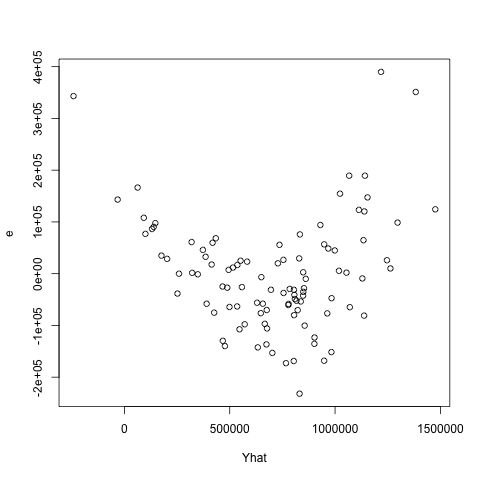
\includegraphics[width=0.5\textwidth]{Yhat_vs_e}
\end{center}

\item 
Now that we know curvature is present, there are two courses of 
action we can take: transform Y or transform the Xj's, or both. 
Generally, if there are problems with the errors, we should transform 
Y, and if the errors are ok, we should transform the Xj's. Let's 
investigate the errors. 

\item 
Plot a qq-plot to check normality of the error terms using the qqnorm 
command. 

\begin{center}
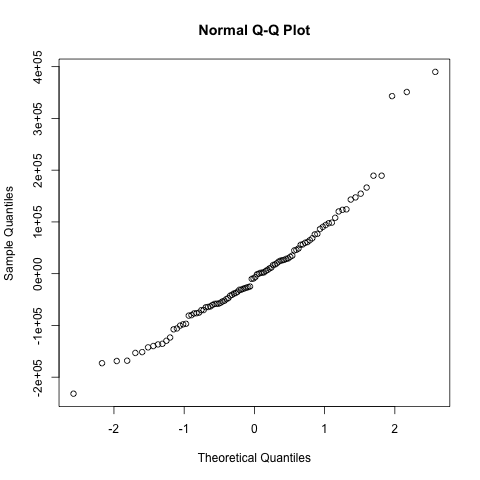
\includegraphics[width=0.5\textwidth]{residuals_qq_plot}
\end{center}
	
\item 
Perform the Shapiro-Wilks test to check normality of the error terms 
using the shapiro.test command.

Using the Shapiro-Wilks test gave a p-value of 0.0002678

\item 
Based on the results in parts (e) and (f), do the error terms for this 
model appear to be normal? 

No. Both the plot and the results of the test give a strong indication that 
the errors are not normally distributed. 

\item 
Check constancy of error variance by plotting $\left|\text{e}\right|$ vs. Yhat. 

\begin{center}
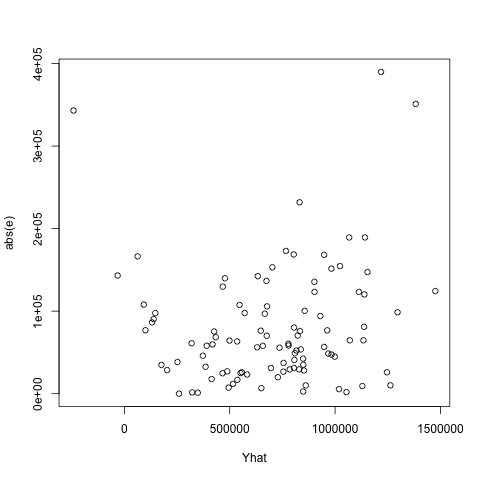
\includegraphics[width=0.5\textwidth]{Yhat_vs_abs_e}
\end{center}
	
\item 
Check constancy of error variance by performing the Brown-Forsythe test. 

The output of this test was: Test Statistic = 1.841, p-value = 0.1779

\item 
Based on the results in parts (h) and (i), do the error terms for this 
model appear to have constant variance? 

No. The Brown-Forsythe test does not have a small p-value, which means that 
the error terms might have constant variance, but the plot does not support 
such an assumption. 

\item 
Does a transformation of Y appear to be necessary? 

Yes.


\item 
Finally, calculate the residual sum of squares $\|e\|^2$. Note that this 
value is 
$\| e \|^2 = \sum (Y_i - \hat{Y}_i)^2, i = 1, ... , n$ 
so it is similar to a prediciton sum of squares. It measures the sum of 
square errors between the predictions Yhati and the actual observations Yi. 
This number is very large, so to put it in perspective, calculate 
\begin{equation}
\frac{
                          \|e\|^2
}{
                       \| Y - \bar{Y}\|^2
}
\end{equation}
       Assessing the model by this criterion is equivalent to using 
\begin{equation}
R^2 = 1 - 
\frac{
                          \|e\|^2
}{
                       \| Y - \bar{Y}\|^2
}
\end{equation}
	The computed sum of squares error is 1.148277e+12

	1 - R2 = 0.09342021

	R2 =  0.9065798
\end{enumerate}

\item 
Let lambda be the optimal value produced by the Box-Cox transformation. 
Transform Y by defining Y.tilde.i = (Y.i)\verb|^|lambda for i = 1, ... , 100.

\begin{enumerate}
\item 
Fit a model tmodel by regressing y.tilde on X1, X2, and X3, and find the 
corresponding fitted values Y.tilde.hat and e.tilde

\item 
Plot Y.tilde vs Y.tilde.hat and e.tilde vs. Y.tilde.hat. How do these plots 
compare to those from problem 2? Does curvature appear to exist in the 
transformed model? 

\begin{center}
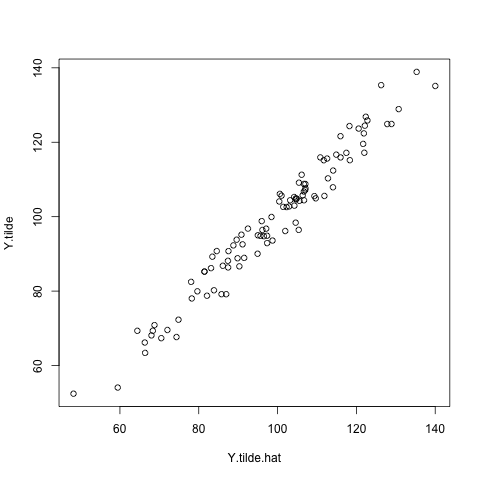
\includegraphics[width=0.5\textwidth]{Ytilde_vs_Ytildehat}
\end{center}
	
\begin{center}
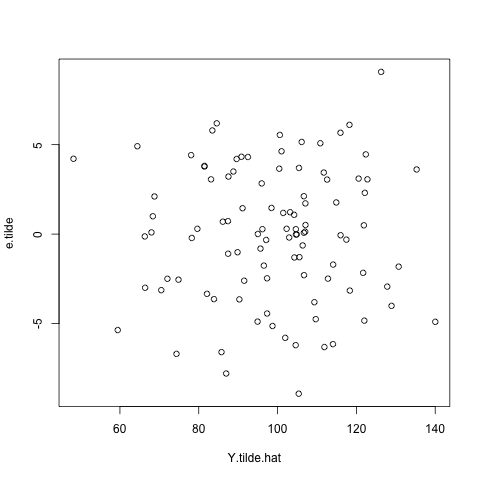
\includegraphics[width=0.5\textwidth]{etilde_vs_Ytildehat}
\end{center}

There does not appear to be any curvature in the transformed model. 
The plot of $\tilde{Y}$ and $\tilde{\hat{Y}}$ is a good indication that 
the predicted values are close to the actual values. There is no 
curvature also, and the residual plot shows random behavior. 

\item 
Investigate normality of the errors for the transformed model. 

\begin{center}
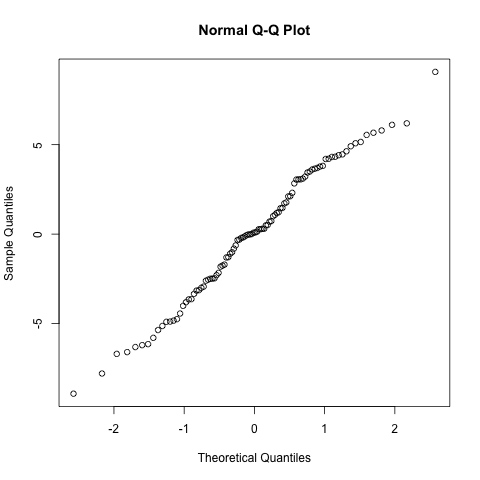
\includegraphics[width=0.5\textwidth]{residuals_qq_plot_t}
\end{center}

The Shapiro-Wilks test gave a p-value of 0.3862 

\item 
Investigate constancy of error variance for the transformed mode. 

\begin{center}
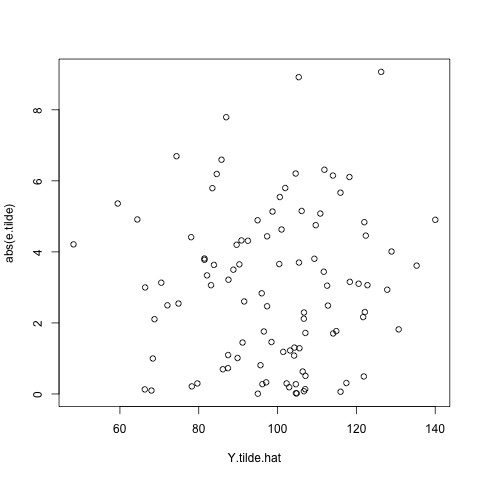
\includegraphics[width=0.5\textwidth]{Yhat_t_vs_abs_e_t}
\end{center}

The results for The Brown-Forsythe test are 
Test Statistic = 0.15792, p-value = 0.6919.

\item 
Do the errors for the transformed model appear to satisfy the assumptions 
of normality and constant error variance? How do your results compare to 
Those from problem 2? 

The Shapiro-Wilks test indicates that the errors are not normal, however, 
looking at the QQ plot, this might be due to the outlier at the upper end. 
This test is very sensitive, and the plot shows very normal behavior except for 
a few outliers near the top of the plot that might skew the results. 

The Brown-Forsythe test again supports the assumption that the errors 
have constant variance. This is also supported be the plot of the errors this time, 
which do display a very constant variance. 

\end{enumerate}

\item 
Now let's apply the results from the transformed model to the original variable Y. 

\begin{enumerate}
\item 
First, create a vector of fitted values for Y by defining 
\begin{Verbatim}
Yhat_i = (Y_tilde_hat_i)^(1 / lambda)
\end{Verbatim}
for i = 1, ... , 100, and create a 
vector of residuals by defining e.i = Yi - Yhati, for i = 1, ..., 100. These 
are predicted values and residuals for the original model, but they take 
advantage of the information from the transformed model. 

\item 
Plot Y vs. Yhat and e vs. Yhat. Did the transformation appear to correct 
problems with the functional form? 

\begin{center}
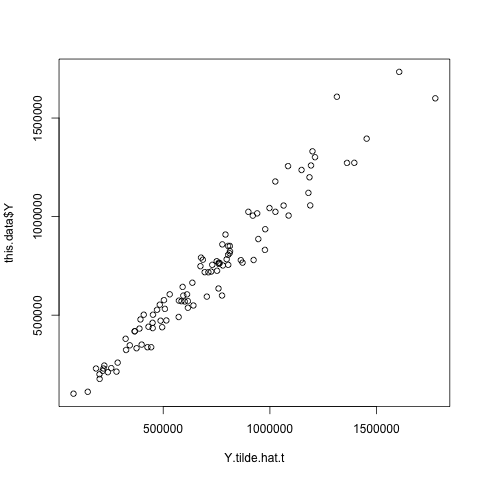
\includegraphics[width=0.5\textwidth]{Y_vs_Ytildehat_t}
\end{center}

\begin{center}
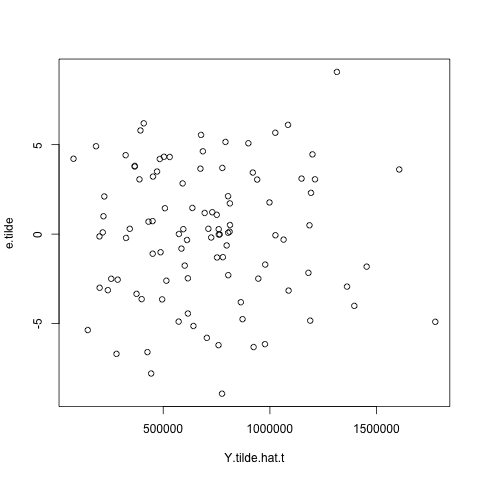
\includegraphics[width=0.5\textwidth]{e_vs_Ytildehat_t}
\end{center}

The transformation does seem to have fixed the problems with the original model. 

\item 
Finally, calculate 
\begin{Verbatim}
||e||2, ||e||2 / (||Y - Ybar||2)
\end{Verbatim}
and 
\begin{Verbatim}
R2 = 1 - ||e||2 / (||Y - Ybar||2)
\end{Verbatim} 
as in question 2. Which model fits the data better/has a lower residual sum of squares? 

The sum of squares error for this model is 1355.552. 

1 - $R^2$ = 1.162408e-10

$R^2$ = 1

The transformed model has the lowest sum of squares error, the better $R^2$ value, and 
appears to satisfy the model assumptions the best. 

\end{enumerate}

\item 
Import the UCI Machine Learning Repository's Auto-MPG data set and create the best 
possible linear regression model for predicting mpg from the other variables. Use 
diagnostics and remedial measures to investigate curvature and assumptions related 
to the design matrix and error terms.

\begin{center}
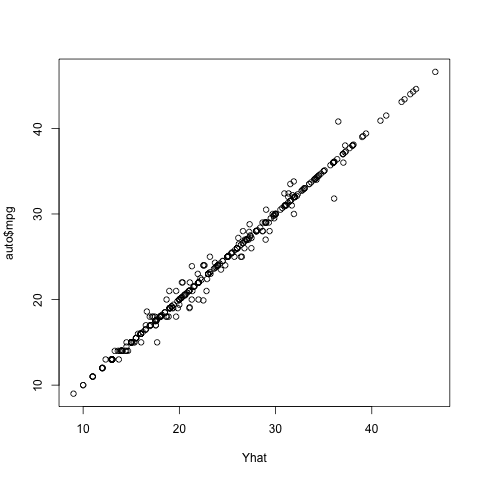
\includegraphics[width=0.5\textwidth]{auto_Yhat_vs_Y}
\end{center}

\begin{center}
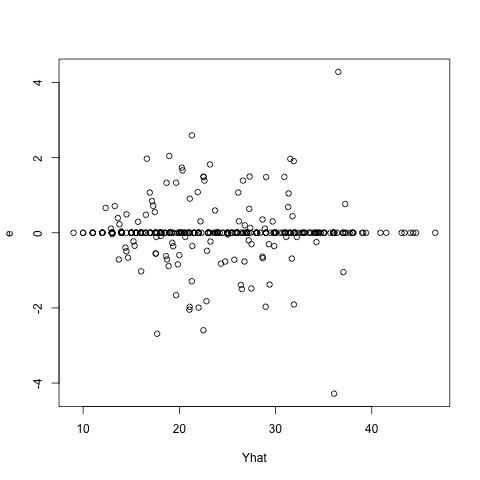
\includegraphics[width=0.5\textwidth]{auto_Yhat_vs_e}
\end{center}

The predicted values match the actual values for mpg very well for this model. There 
does not appear to be any curvature involved in this case. Instead of having a random 
and evenly distributed range of values about $0$, the residual plot shows a strong bias 
to $0$. This is supported also by the QQ plot for residuals shown below. 

\begin{center}
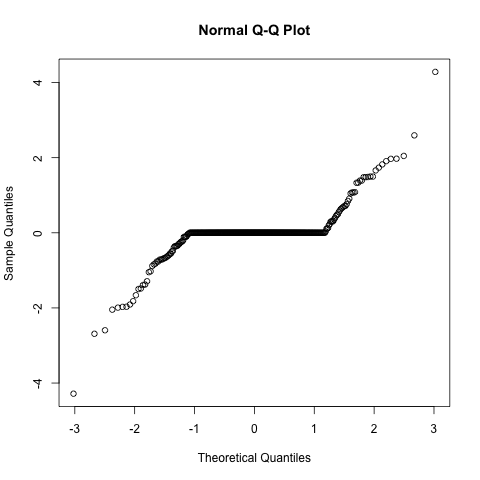
\includegraphics[width=0.5\textwidth]{auto_residuals_qq_plot}
\end{center}

The errors do not appear to be normally distributed. The Shapiro-Wilks test 
gave a p-value $ < 2.2e-16$, suggesting very strongly that the residuals are not 
normally distributed. 

The Brown-Forsythe test gave the following results for this model: 

Test Statistic = 0.0026272, p-value = 0.9591

The plot of $\hat{Y}$ vs residuals is shown below. This shows very strongly the 
errors do not have constant variance. 

\begin{center}
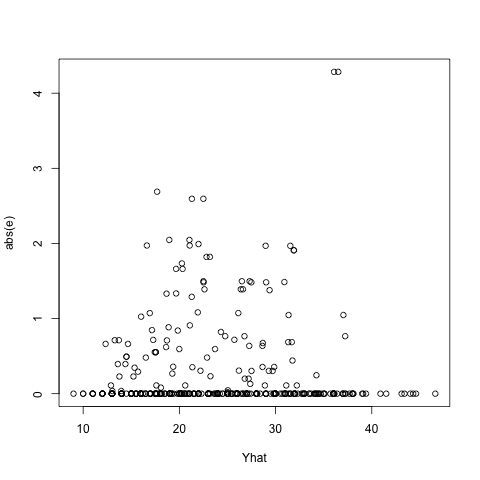
\includegraphics[width=0.5\textwidth]{auto_Yhat_vs_abs_e}
\end{center}

The sum of squares error for this model is 159.0592. The $R^2$ statistic is $\approx$ 1, and 
$1 - R^2$ is 1.294054e-11. 

\end{enumerate}
\pagebreak
\lstinputlisting[language=R, basicstyle=\ttfamily\scriptsize]{hw23.R}
\end{document}
